%%%%%%%%%%%%%%%%%%%%%%%%%%%%%%%%%%%%%%%%%%%%%%%%%%%%%%%%%%%%%%%%%%%%%%%%%%%%%%%%
%2345678901234567890123456789012345678901234567890123456789012345678901234567890
%        1         2         3         4         5         6         7         8

\documentclass[letterpaper, 10 pt, conference]{ieeeconf}  % Comment this line out
                                                          % if you need a4paper
%\documentclass[a4paper, 10pt, conference]{ieeeconf}      % Use this line for a4
                                                          % paper

\IEEEoverridecommandlockouts                              % This command is only
                                                          % needed if you want to
                                                          % use the \thanks command
\overrideIEEEmargins
% See the \addtolength command later in the file to balance the column lengths
% on the last page of the document



% The following packages can be found on http:\\www.ctan.org
%\usepackage{graphics} % for pdf, bitmapped graphics files
%\usepackage{epsfig} % for postscript graphics files
%\usepackage{mathptmx} % assumes new font selection scheme installed
%\usepackage{times} % assumes new font selection scheme installed
%\usepackage{amsmath} % assumes amsmath package installed
%\usepackage{amssymb}  % assumes amsmath package installed

\usepackage{cmap}					% поиск в PDF
\usepackage{mathtext} 				% русские буквы в формулах
\usepackage[T2A]{fontenc}			% кодировка
\usepackage[utf8]{inputenc}			% кодировка исходного текста
\usepackage[english,russian]{babel}	% локализация и переносы
\usepackage {algorithmic}
%\usepackage []{algorithm2e}
\usepackage {graphicx}
%\usepackage {program}

\title{\LARGE \bf
Определение местоположения по сигналам акселерометра
}

%\author{ \parbox{3 in}{\centering Huibert Kwakernaak*
%         \thanks{*Use the $\backslash$thanks command to put information here}\\
%         Faculty of Electrical Engineering, Mathematics and Computer Science\\
%         University of Twente\\
%         7500 AE Enschede, The Netherlands\\
%         {\tt\small h.kwakernaak@autsubmit.com}}
%         \hspace*{ 0.5 in}
%         \parbox{3 in}{ \centering Pradeep Misra**
%         \thanks{**The footnote marks may be inserted manually}\\
%        Department of Electrical Engineering \\
%         Wright State University\\
%         Dayton, OH 45435, USA\\
%         {\tt\small pmisra@cs.wright.edu}}
%}

\author{Зайнулина~Э.\,Т., Киселёва~Е.\,А.,Фатеев~Д.\,А.,
    Божедомов~Н.,
    Протасов~В.% <-this % stops a space
\thanks
    {
   Научный руководитель:  Стрижов~В.\,В.
    Консультант:  Мотренко~А.}
    }


\begin{document}



\maketitle
\thispagestyle{empty}
\pagestyle{empty}


%%%%%%%%%%%%%%%%%%%%%%%%%%%%%%%%%%%%%%%%%%%%%%%%%%%%%%%%%%%%%%%%%%%%%%%%%%%%%%%%
\begin{abstract}
Cистемы внутреннего и наружного позиционирования играют важную роль в современном мире. Для определения места положения используются Глобальные системамы позиционирования (GPS); однако, не всегда есть возможность воспользоваться ими.

В данной статье предложен метод увеличения точности отслеживания человека по сигналам акселерометра, гироскопа и магнитометра.

Чтобы увеличить точность и уменьшить время вычислений, мы используем модель PDR (pedestrian dead reckoning). Так как данные неизбежно собираются с некоторым шумом, применяем Гауссовское сглаживание. Задача исследования ставится в терминах Projection to Latent Spaces, т.к. восстановление траектории происходит целиком, а не от точки к точке.
\end{abstract}
\begin{keywords}
PDR, PLS, Position system, User location.
\end{keywords}

%%%%%%%%%%%%%%%%%%%%%%%%%%%%%%%%%%%%%%%%%%%%%%%%%%%%%%%%%%%%%%%%%%%%%%%%%%%%%%%%
\section{ВВЕДЕНИЕ}
Определение местонахождения человека черезвычайно важная задача. Мы пользуемся системами GNNS, чтобы не потерться в городе или добраться до соседнего, обеспечить безопасность в толпе, координировать действия рабочих. Но GNNS определяет местоположение в здании неточно.

Методы основанные на сигналах WiFi, Bluetooth, UWB [7][12] требуют дополнительной информации: карты помещения или набора ключевых точек. Это не всегда удобно или даже реализуемо.

С другой стороны сейчас у каждого человека в кармане целый арсенал средств для ориентирования в пространстве. Все спрятано в наших смартфонах: акселерометр, гироскоп, магнитометр. В нашей работе мы предлагаем восстанавливать полную траекторию по сигналам этих датчиков, используя модель PDR, избавляясь от зашумленности с помощью Гауссовского сглаживания.


\section{ПОСТАНОВКА ЗАДАЧИ}

\subsection{Модель}

$$ \mathrm{f}  : \mathrm{X}   \rightarrow \mathrm{Y}$$

$\mathrm{X} \in \mathbb{R}^{N \times T} $ - матрица признаков, 

$\mathrm{Y} \in \mathbb{R}^{2 \times T}$  - траектория пешехода

$y(t)  $ - строки матрицы $\mathbb{Y}$,  временные ряды, описывающие изменения глобальных координатпешехода во времени.

\subsection{Подзадачи}

\begin{enumerate}
\item Определение класса местоположения датчика: рука, нога, сумка, тело.
\item  Предсказании траектории на основе полученного класса\[f \to f_1 ~ f_2\]
\[f_1: X \to P = \{0, 1, 2, 3\}\]
\[f_2: X, ~P \to Y\]
\end{enumerate}

\subsection{Методы}

Используем метод опорных векторов для классификации и регрессии.

Минимизируем $S(w|f, X, Y)$:

\[\min_{w, w_0}S(w, w_0) = \|w\|^2+C\sum_{i}\xi_i\]
\[subject~to~y_i(w^Tx_i+w_0)\geq 1-\xi_i\]
\[\xi_i \geq 0~\forall i\] 

$S(w, w_0)$ - штраф за суммарную ошибку.

\subsection{Оценка качества модели}

Используем критерий суммы квадратов отклонений предсказанных координат от истинных, корреляция между предсказанной и истинной траекториями пешехода.

\[w^* = \arg\min_{w}S(w|f, X, Y).\]


\section{БАЗОВАЯ МОДЕЛЬ}
\begin{itemize}

\item Чтобы устранить зашумленность данных применяем Гауссовское сглаживание для 6 каналов гиростабилизатора и 2 скоростных каналов. Полученные скорости преобразуем в вектор признаков.
\item Строим матрицу признаков X.
\item С помощью матрицы X и SVM-классификатора определяем, где находится датчик. (Рука, нога, сумка, тело).
\item Для каждого класса обучаем 2 SVMR-регрессора. Первый определяет скорости движения человека в разные промежутки времени и угловые скорости для канала X. Но эти результаты имеют ошибку из-за неточности датчиков гироскопа, акселерометра. Решаем задачу минимизации этой ошибки.

\[\min_{\{x^1_I, x^51_I,\dots\}}V_{bias}=
\min_{\{x^1_I, x^51_I,\dots\}}\sum_{f \in F_2}\|v_C^F-v_R^f\|+
\lambda\sum_{f \in F_1}\|x^f_I\|^2,\]
\[v_C^f = R_{SW}^f\sum_{f'=1}^f R_{WI}^{f'}(a_I^{f'}+x_I^{f'}),\]
где $f$ - единица блока выборки, $F$ - блок выборки, $v_C^F$ - скорректированное значение скорости, $v_R^f$ - предсказанное значение скорости, $I$ - система координат устройства, $W$ - глобальная система координат, $S$ - IMU-стабилизированная система координат, $R_{AB}$ - матрица перехода из системы координат $B$ в систему координат $A$.

Второй предсказывает то же для 2 канала.

\item По полученным скоростям восстанавливаем траекторию пешехода.
\item Алгоритм:

\begin{algorithmic}[1]
\REQUIRE $X, Y_{class}, Y, X_{test}$
\STATE $initialize ~ classifier\_options$
\STATE $classifier = SVMClassifier(classifier\_options);$
\STATE $classifier.fit(X, Y_{class})$
\FOR {$cls ~ in ~ classes$:}
\STATE $initialize ~ regressor\_cls\_optons$
\STATE $regressor\_cls = SVRRegressor(regressor\_cls\_optons)$
\STATE $regressor\_cls.fit(X[X[ind] \in cls], Y)[Y[ind] \in cls])$
\ENDFOR
\STATE $Y_{test-class} = classifier.predict(X_{test})$
\FOR {$cls ~ in ~ classes$:}
\STATE $Velocity\_cls = regressor\_cls.predict(X_{test} [Velocity\_class[ind] == cls]$
\STATE $x^1_I, x^51_I,\dots = \argmin_{\{x^1_I, x^51_I,\dots\}}V_{bias}\_cls$
\STATE $Velocity\_cls = R_{SW}^f\sum_{f'=1}^f R_{WI}^{f'}(a_I^{f'}+x_I^{f'})$
\STATE $Trajectory\_cls$ recovery depending on $Velocity\_cls$
\ENDFOR
\RETURN $Full\_trajectory$
\end{algorithmic}

\end{itemize}


\section{БАЗОВЫЙ ЭСПЕРИМЕНТ}
Для эксперимента используется часть данных, собранных в статье, описывающей алгоритм RIDI [7]. Эти данные были получены с помощью инерционных датчиков, расположенных в смартфонах в нескольких случаях: когда смартфон располагался на поясе, в руке, на ноге или в сумке. Выборки содержат различные траектории длиной в 100 минут и частотой сигнала 200 Гц. В качестве объекта рассматривается положение в определенный момент времени $i$ Признаками объекта являются угловые скорости и линейные ускорения в стабилизированной системе координат датчиков в моменты времени $i - window_size$, $Window_size$ - размер окна (равен 200). Целевыми переменными
являются метки классов, характеризующие то, в каком положении находился смартфон при получении определенных данных, а также скорости в данный момент времени $i$, которые вычисляются через координаты пешехода и прошедшее время. По полученным данным после уточнения скоростей с помощью оптимизации функции  строится
предсказанная траектория пешехода.

\subsection{Графики зависимости качества предсказания модели от параметров}

\begin{enumerate}
    \item Выборка 1 состоит из 30742 объектов (8728 объектов класса рука, 6106 объектов класса нога, 7758 объектов класса тело, 8150 объектов класса сумка).
    
    \item Выборка 2 состоит из 42731 объектов (13204 объектов класса рука, 8083 объектов класса нога, 11105 объектов класса тело, 10339 объектов класса сумка).
    
    \item Выборка 3 состоит из 35892 объектов (9458 объектов класса рука, 7304 объектов класса нога, 13306 объектов класса тело, 5824 объектов класса сумка).
    
\end{enumerate}
    
см. Fiag. 1- 8
    
    \begin{figure}[H]
    \includegraphics[scale=0.2]{charts/handheld_chn0_C=10.pdf}
    \caption{Рука, канал 0}
    \label{fig:image}
    \end{figure}
    
    \begin{figure}[H]
    \includegraphics[scale=0.2]{charts/handheld_chn1_C=10.pdf}
    \caption{Рука, канал 1}
    \label{fig:image}
    \end{figure}
    
    \begin{figure}[H]
    \includegraphics[scale=0.2]{charts/leg_chn0_C=10.pdf}
    \caption{Нога, канал 0}
    \label{fig:image}
    \end{figure}
    
    \begin{figure}[H]
    \includegraphics[scale=0.2]{charts/leg_chn1_C=10.pdf}
    \caption{Нога, канал 1}
    \label{fig:image}
    \end{figure}
    
    \begin{figure}[H]
    \includegraphics[scale=0.2]{charts/bag_chn0_C=10.pdf}
    \caption{Сумка, канал 0}
    \label{fig:image}
    \end{figure}
    
    \begin{figure}[H]
    \includegraphics[scale=0.2]{charts/bag_chn1_C=10.pdf}
    \caption{Сумка, канал 1}
    \label{fig:image}
    \end{figure}
    
    \begin{figure}[H]
    \includegraphics[scale=0.2]{charts/body_chn0_C=10.pdf}
    \caption{Тело, канал 0}
    \label{fig:image}
    \end{figure}
    
    \begin{figure}[H]
    \includegraphics[scale=0.2]{charts/body_chn1_C=10.pdf}
    \caption{Тело, канал 1}
    \label{fig:image}
    \end{figure}

\subsection{Оптимальные параметры эксперимента}
см. Table I
\begin{table}[H]
\caption{Table 1}
\begin{center}
\begin{tabular}{|c|c|c|c|c|}
\hline
& Рука & Нога & Сумка & Тело \\
\hline
C & 10 & 1 & 1 & 1 \\
\hline
$\gamma$ & 0.01 & 0.001 & 0.01 & 0.001\\
\hline
\end{tabular}
\end{center}
\end{table} 


\subsection{Результаты}
см. Fig.9-10
\begin{figure}[h]
\begin{minipage}[h]{0.49\linewidth}
\center{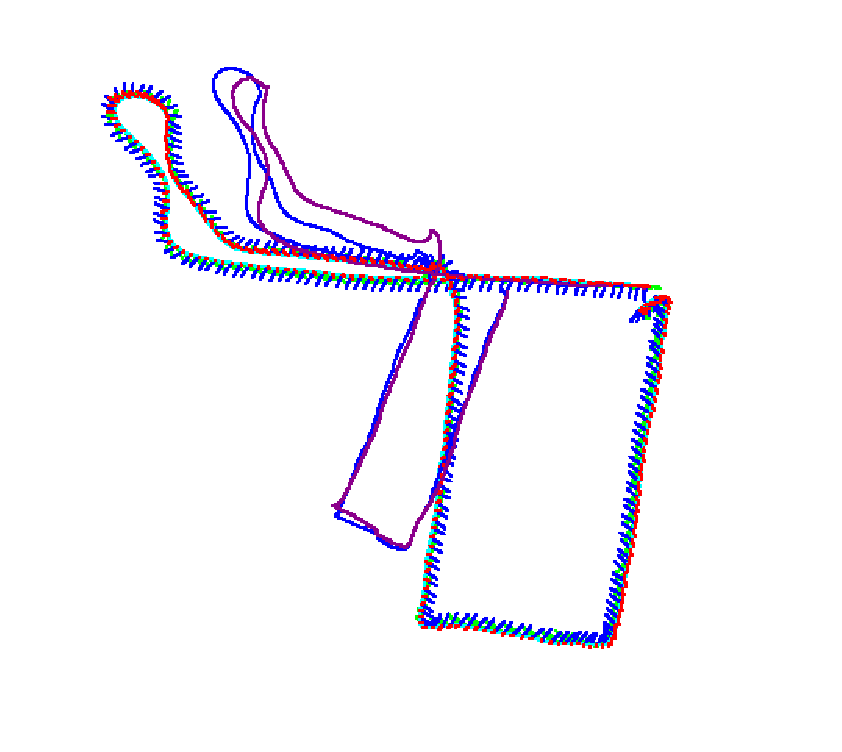
\includegraphics[width=0.5\linewidth]{trajectories/zhicheng_bag00.eps} \\ Класс-сумка}
\end{minipage}
\hfill
\begin{minipage}[h]{0.49\linewidth}
\center{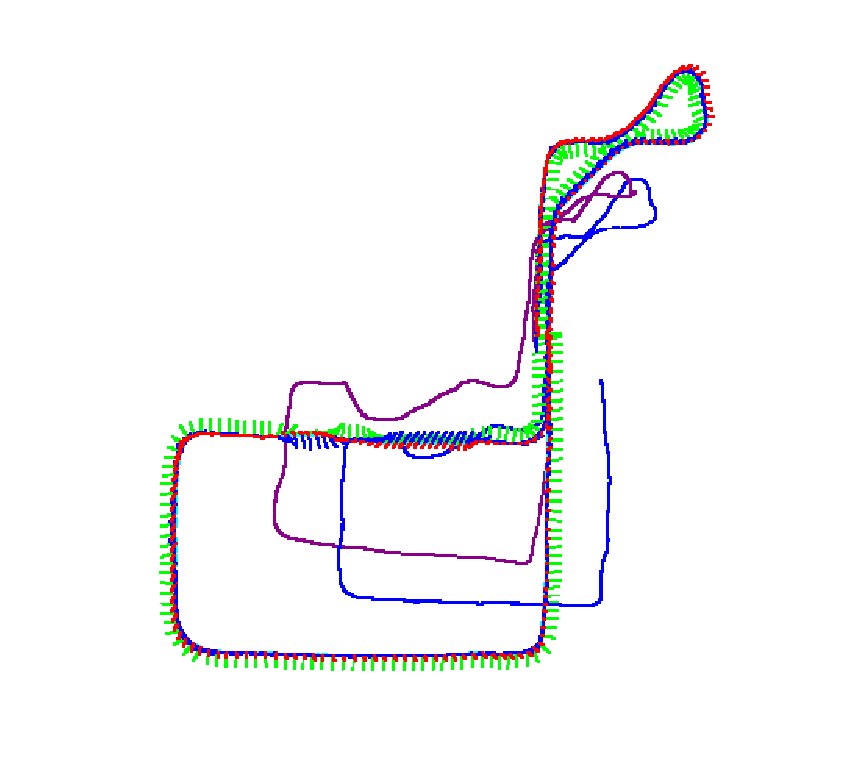
\includegraphics[width=0.5\linewidth]{trajectories/zhicheng_handheld00.eps} \\ Класс-рука}
\end{minipage}
\caption{Траектории}
\label{ris:image1}
\end{figure}

\begin{figure}[h]
\begin{minipage}[h]{0.49\linewidth}
\center{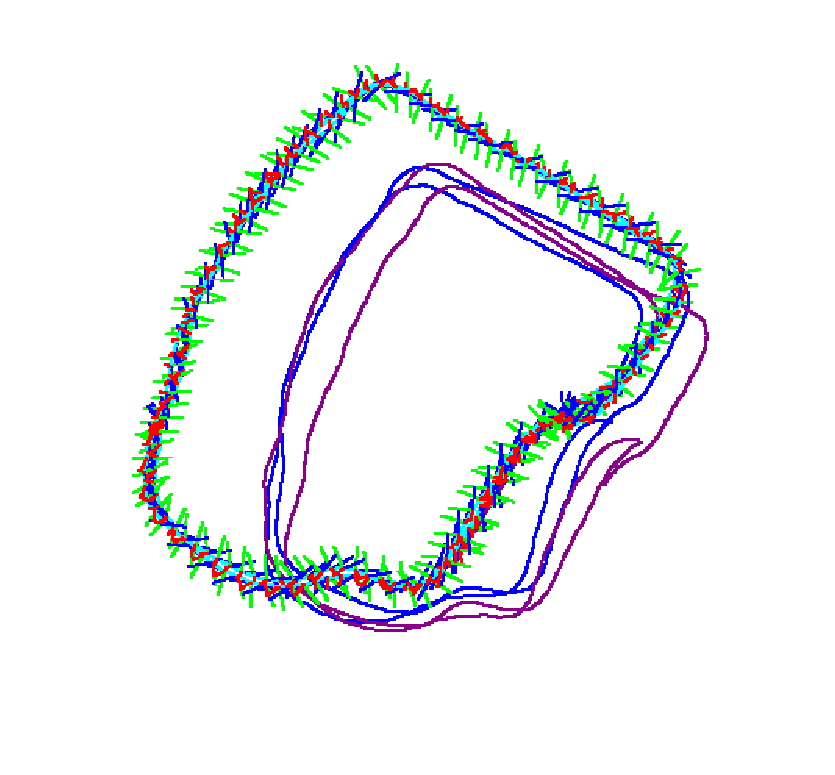
\includegraphics[width=0.5\linewidth]{trajectories/zhicheng_leg00.eps} \\ Класс-нога}
\end{minipage}
\caption{Траектории}
\end{figure}


\section{ВЫВОДЫ}

 Повторив эксперимент статьи [7] мы убедились, что классификация нахождения датчика (рука, нога, сумка, тело) повышает точность предсказания траектории. Убедились, что для устранения шума лучше использовать фильтр Гаусса. 

\addtolength{\textheight}{-12cm}   % This command serves to balance the column lengths
                                  % on the last page of the document manually. It shortens
                                  % the textheight of the last page by a suitable amount.
                                  % This command does not take effect until the next page
                                  % so it should come on the page before the last. Make
                                  % sure that you do not shorten the textheight too much.

%%%%%%%%%%%%%%%%%%%%%%%%%%%%%%%%%%%%%%%%%%%%%%%%%%%%%%%%%%%%%%%%%%%%%%%%%%%%%%%%



%%%%%%%%%%%%%%%%%%%%%%%%%%%%%%%%%%%%%%%%%%%%%%%%%%%%%%%%%%%%%%%%%%%%%%%%%%%%%%%%



%%%%%%%%%%%%%%%%%%%%%%%%%%%%%%%%%%%%%%%%%%%%%%%%%%%%%%%%%%%%%%%%%%%%%%%%%%%%%%%%

\section*{ACKNOWLEDGMENT}




\begin{thebibliography}{99}

\bibitem{c1} Erich Bruns and Oliver Bimber. Adaptive training of video sets for image recognition on mobile
phones. Personal and Ubiquitous Computing, 13(2):165–178, 2009.
\bibitem{c2}L. Chen, E. H. Wu, M. Jin, and G. Chen. Intelligent fusion of wi-fi and inertial sensor-based
positioning systems for indoor pedestrian navigation. IEEE Sensors Journal, 14(11):4034–4042,
Nov 2014.
\bibitem{c3} Fr´ed´eric Evennou and Fran¸cois Marx. Advanced integration of wifi and inertial navigation systems
for indoor mobile positioning. EURASIP J. Adv. Sig. Proc, 2006, 2006.
\bibitem{c4} Michael Hardegger, Daniel Roggen, and Gerhard Tr¨oster. 3d actionslam: wearable person tracking
in multi-floor environments. Personal and Ubiquitous Computing, 19(1):123–141, 2015.
\bibitem{c5} R. Hostettler and S. S¨arkk¨a. Imu and magnetometer modeling for smartphone-based pdr. In 2016
International Conference on Indoor Positioning and Indoor Navigation (IPIN), pages 1–8, Oct
2016.
\bibitem{c6} W. Kang and Y. Han. Smartpdr: Smartphone-based pedestrian dead reckoning for indoor
localization. IEEE Sensors Journal, 15(5):2906–2916, May 2015.
\bibitem{c7} Hang Yan, Qi Shan, and Yasutaka Furukawa. Ridi: Robust imu double integration. CoRR,
abs/1712.09004, 2017.

\end{thebibliography}




\end{document}
